\begin{frame}{What is a signal?}
\begin{block}{Our definition}
Function (or something that can be represented as) that contains information about the behavior or attributes of some phenomenon. It can be digital (discrete) or analog (continuous).
\end{block}
\pause
\begin{figure}[!tbp]
  \centering
  \begin{minipage}[b]{0.45\textwidth}
    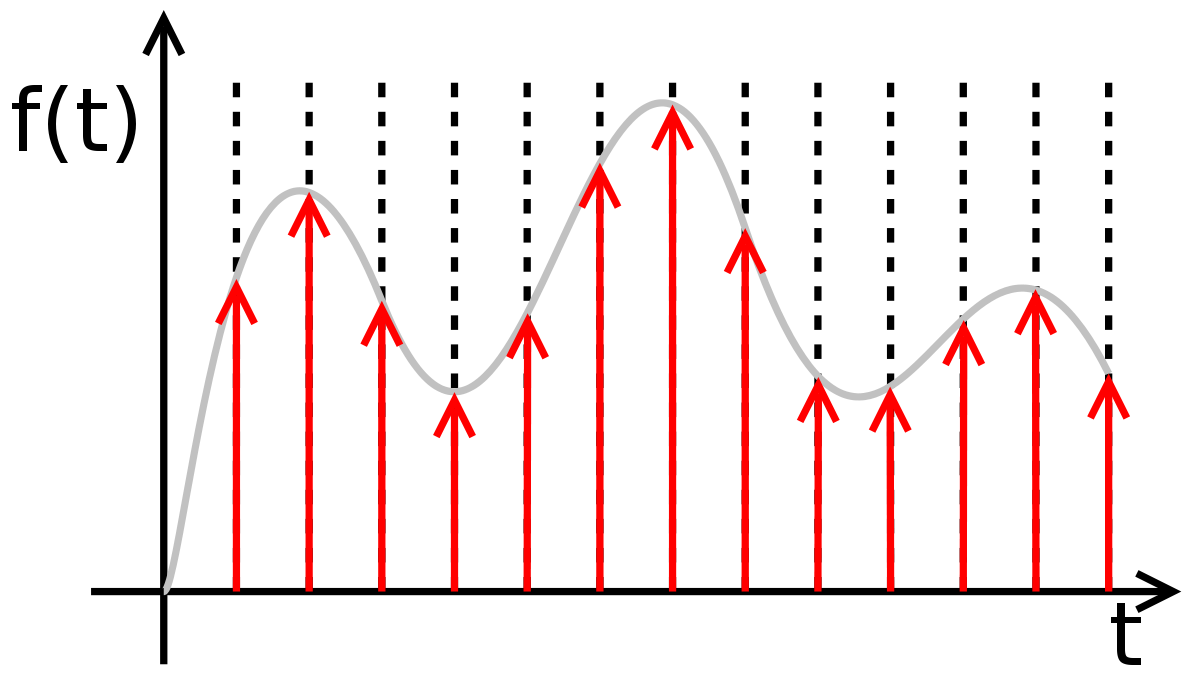
\includegraphics[width=\textwidth]{./Images/digita_signal.png}
    \caption{Digital and continuous one-dimensional signals}
  \end{minipage}
	\pause
  \hfill
  \begin{minipage}[b]{0.45\textwidth}
    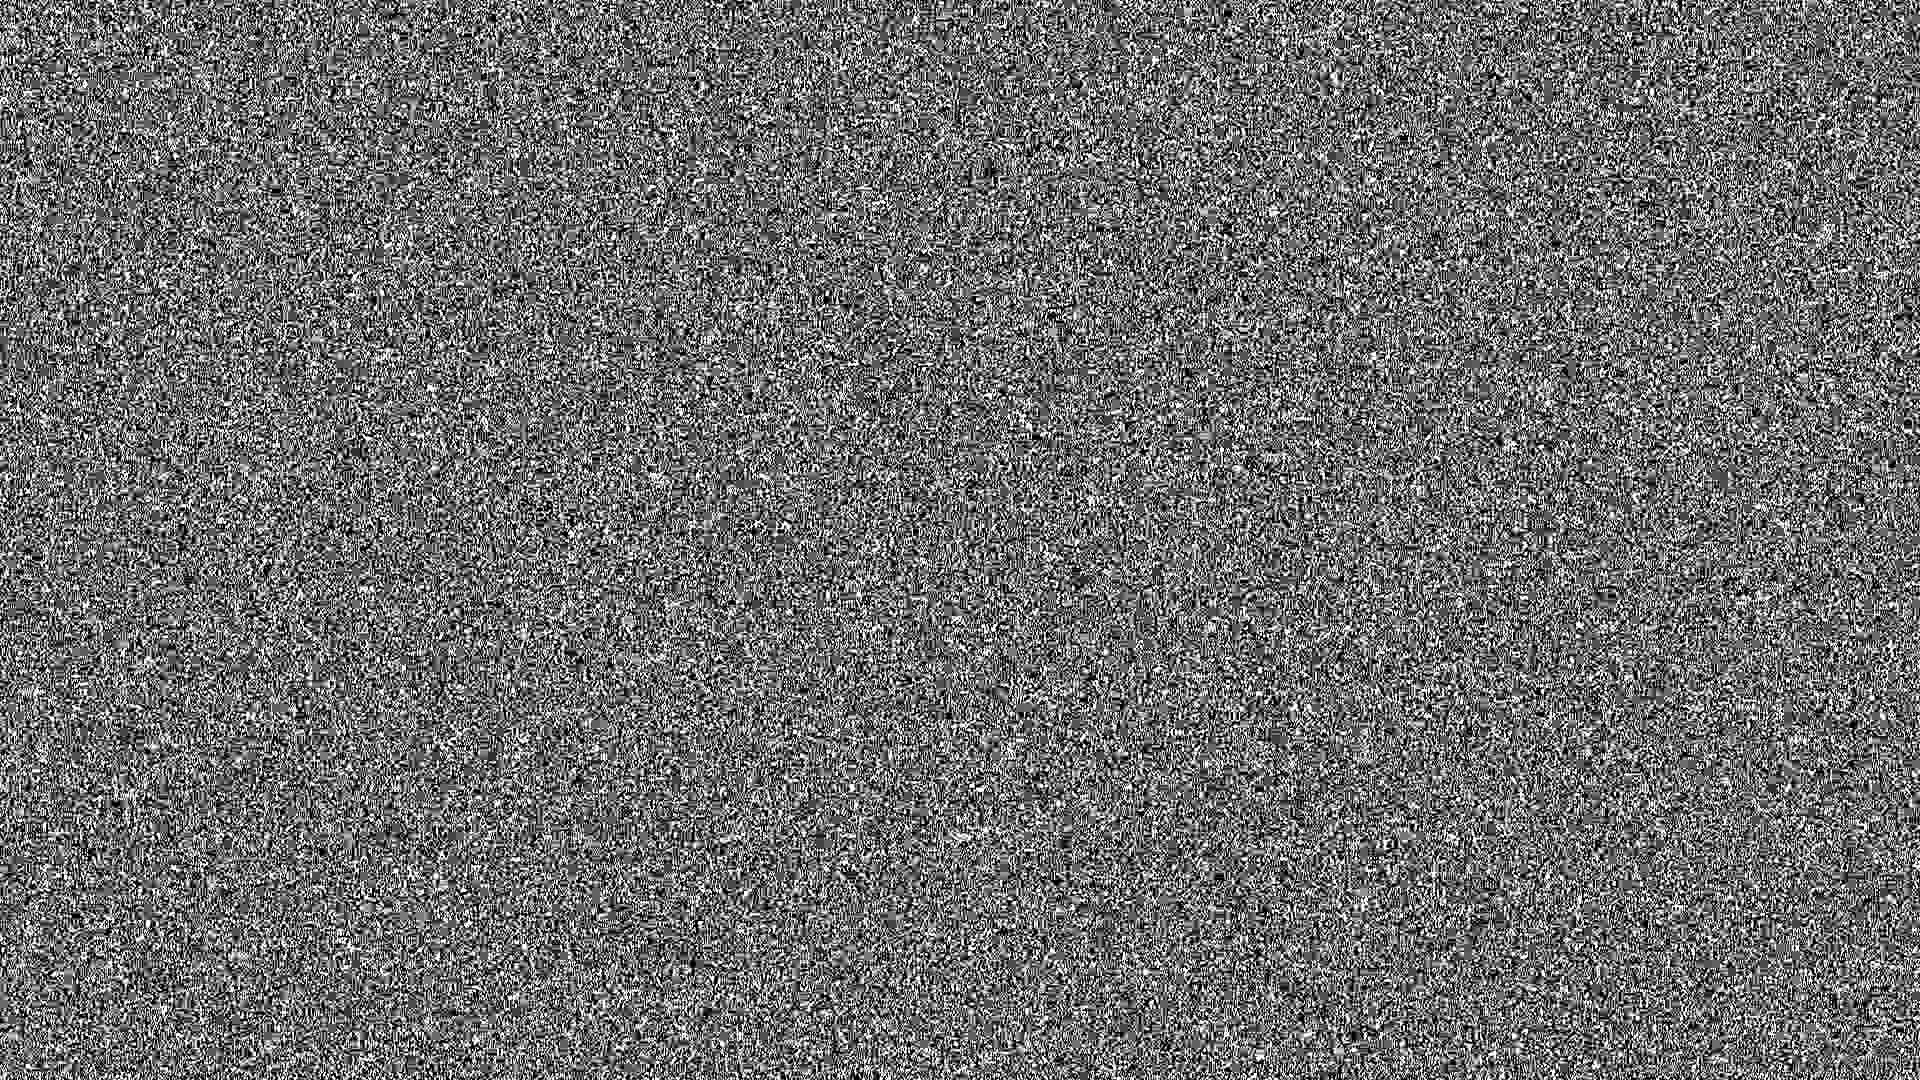
\includegraphics[width=\textwidth]{./Images/white_noise.jpg}
    \caption{White noise, not a signal}
  \end{minipage}
\end{figure}
\end{frame}

\begin{frame}{Sparse representations of signals}
\begin{itemize}
 \item Relevant information in structured data is sparse, due the high correlation of its elements.\pause
 \item Goal: Find the right dictionary to represent optimally our data.
\end{itemize}
\begin{figure}[h!]
\centering
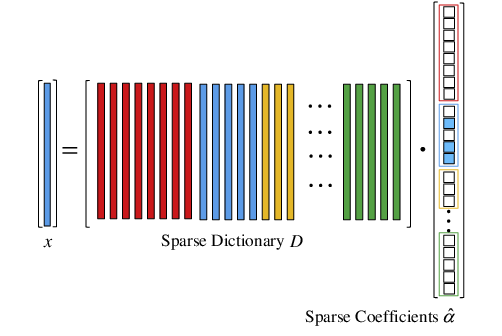
\includegraphics[width=0.7\textwidth]{./Images/sparse_data.png}
\end{figure}
\end{frame}

\begin{frame}{Fourier Transform (Fourier, 1822)}
$$
\hat{f}(\omega):=\int_{\mathbb{R}^n} f(x)e^{-i\langle x,\omega\rangle} dx
$$
\pause
\begin{figure}[h!]
\centering
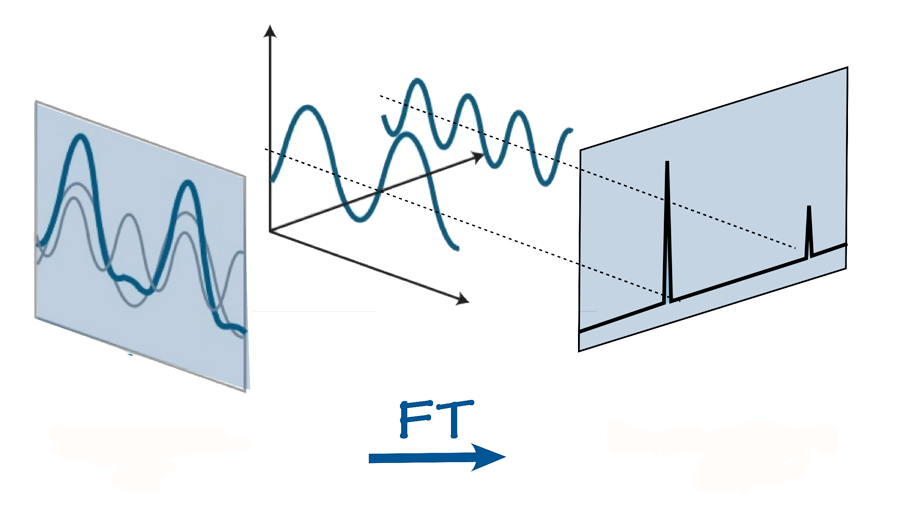
\includegraphics[width=0.7\textwidth]{./Images/fourier.png}
\end{figure}
\end{frame}

\begin{frame}{Short Time Fourier Transform (Gabor,1946)}
$$
S_gf(t,\omega)=\int_{\mathbb{R}} f(x)\overline{g(x-t)}e^{-ix\omega}dx
$$
\pause
\begin{figure}[h!]
\centering
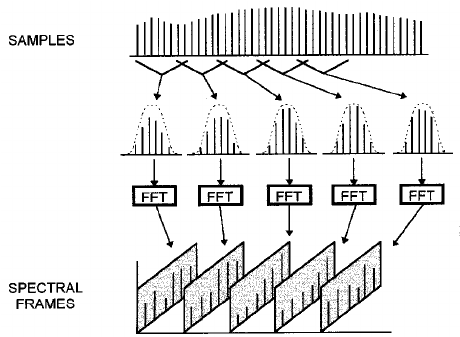
\includegraphics[width=0.68\textwidth]{./Images/STFT.png}
\end{figure}
\end{frame}

\begin{frame}{Wavelet Transform (Morlet and Grossman, 1984)}
$$
\begin{aligned}
\mathcal{W}_{\psi}f(a,b)&=\int_{\mathbb{R}}f(t)a^{-\frac{1}{2}}\overline{\psi\left(\frac{t-b}{a}\right)}dt\\
&=(f\ast D_a\overline{\psi}^*)(b)\textrm{,}\quad (a, b)\in\mathbb{R}^+\times\mathbb{R}
\end{aligned} 
$$
where 
$$
\int_0^{\infty}\frac{|\hat{\psi}(\omega)|^2}{\omega}d\omega<\infty
$$
\pause
\begin{figure}[h!]
\centering
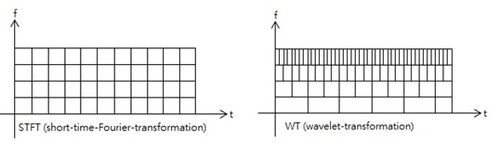
\includegraphics[width=1\textwidth]{./Images/wavelet.jpg}
\end{figure}
\end{frame}

\begin{frame}{Cartoon-like functions}
\begin{definition}
Let $f:\mathbb{R}^2\longrightarrow\mathbb{C}$, $f\in\mathcal{E}^2(\mathbb{R}^2)$ if $f= f_0+\chi_B f_1$, with $B\subset [0,1]^2$, $\partial B\in C^2$ and with bounded curvature. Moreover, $f_i\in C^2(\mathbb{R}^2)$ with $||f_i||_{C^2}\leq 1$ and $\text{supp} f_i\subset [0,1]^2$ for $i=0,1$. 
\end{definition}
\pause
\begin{figure}[h!]
\centering
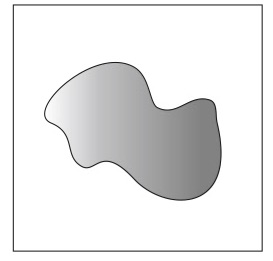
\includegraphics[width=0.4\textwidth]{./Images/cartoon-like.jpg}
\end{figure}
\end{frame}

\begin{frame}{Optimal error for 2D signals}
\begin{block}{Best N-term approx.\ error (Donoho, 2001)}
Let $\{\psi_{\lambda}\}_{\lambda\in\Lambda}\subset L^2(\mathbb{R}^2)$ a frame. The optimal best N-Term approximation error for any $f\in\mathcal{R}^2(\mathbb{R}^2)$ is
$$
\sigma_N(f,\{\psi_{\lambda}\}_{\lambda\in\Lambda})=O(N^{-1})
$$
\end{block}
\pause
\begin{block}{Error of 2D-wavelets}
$$
\sigma_N(f,\{\psi_{j,m}\}_{j,m})\sim N^{-1/2}
$$
\end{block}
\pause
\begin{figure}[h!]
\centering
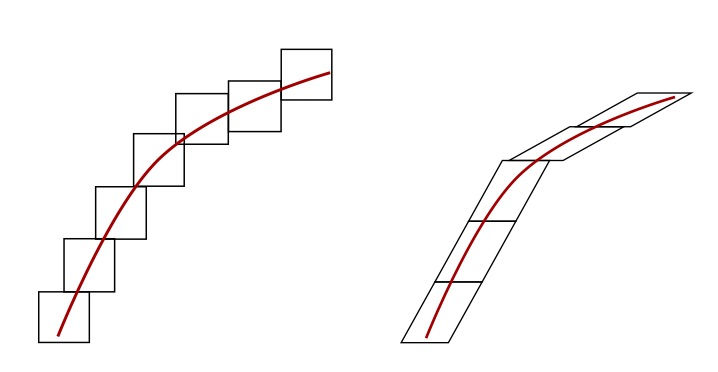
\includegraphics[width=0.4\textwidth]{./Images/anisotropic_isotropic.jpg}
\end{figure}
\end{frame}

\begin{frame}{How to solve this? Scaling and Shearing}

\begin{minipage}{0.25\textwidth}
\begin{itemize}
\item\textit{Scaling}
$$
A_j:=
\left(
\begin{matrix}
2^j & 0 \\
0 & 2^{j/2}
\end{matrix}
\right)
$$
\end{itemize}
\end{minipage}  \hfill
\pause
\begin{minipage}{0.65\textwidth}
\begin{figure}[!tbp]
  \centering
  \begin{minipage}[b]{0.45\textwidth}
    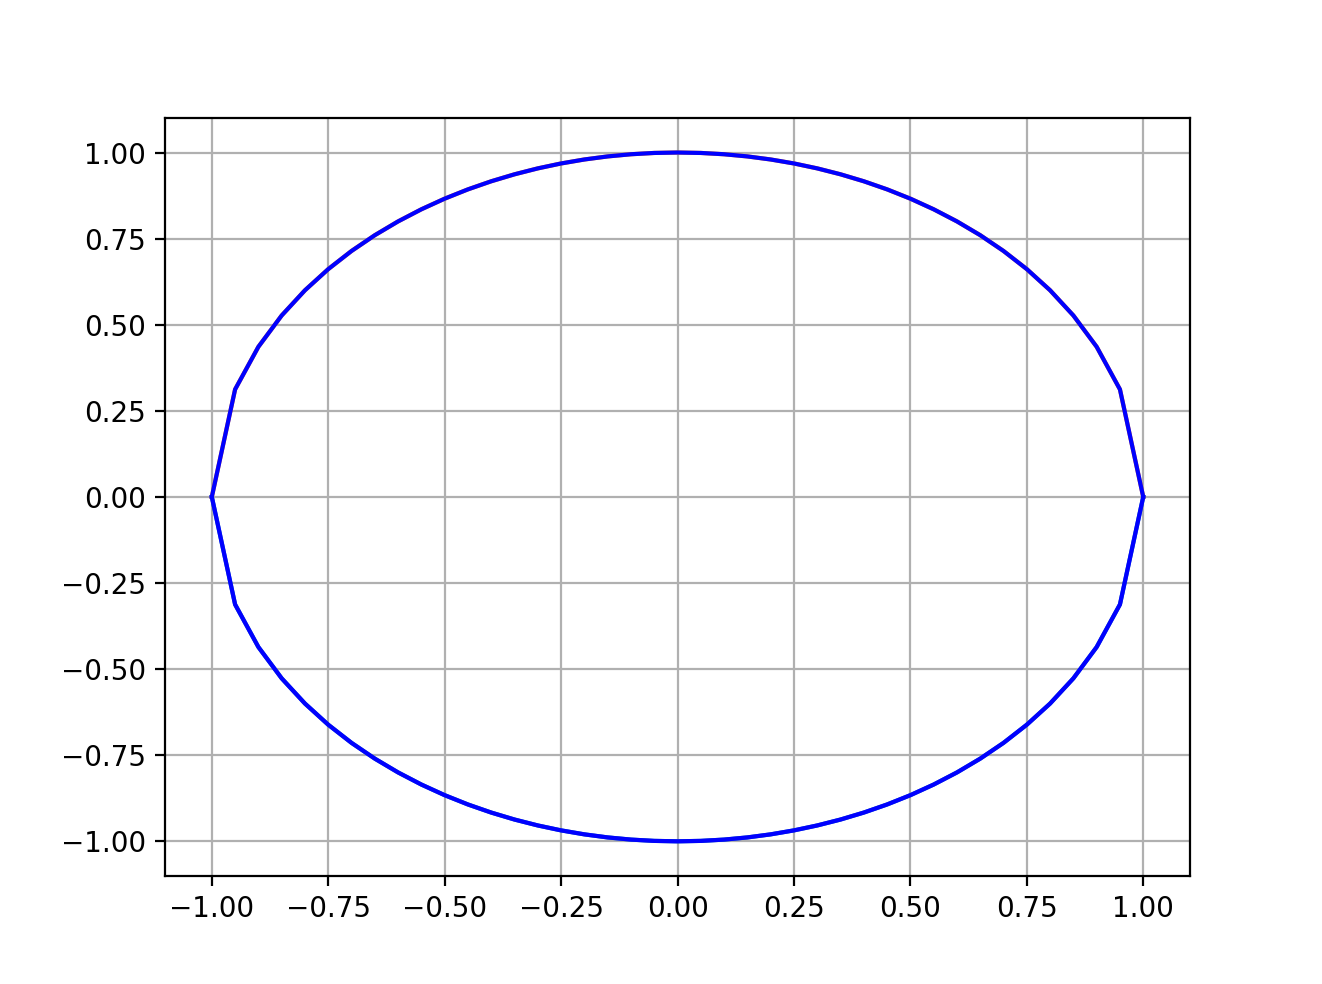
\includegraphics[width=\textwidth]{./Images/circle.png}
  \end{minipage}
	\pause
 \hfill 
  \begin{minipage}[b]{0.45\textwidth}
    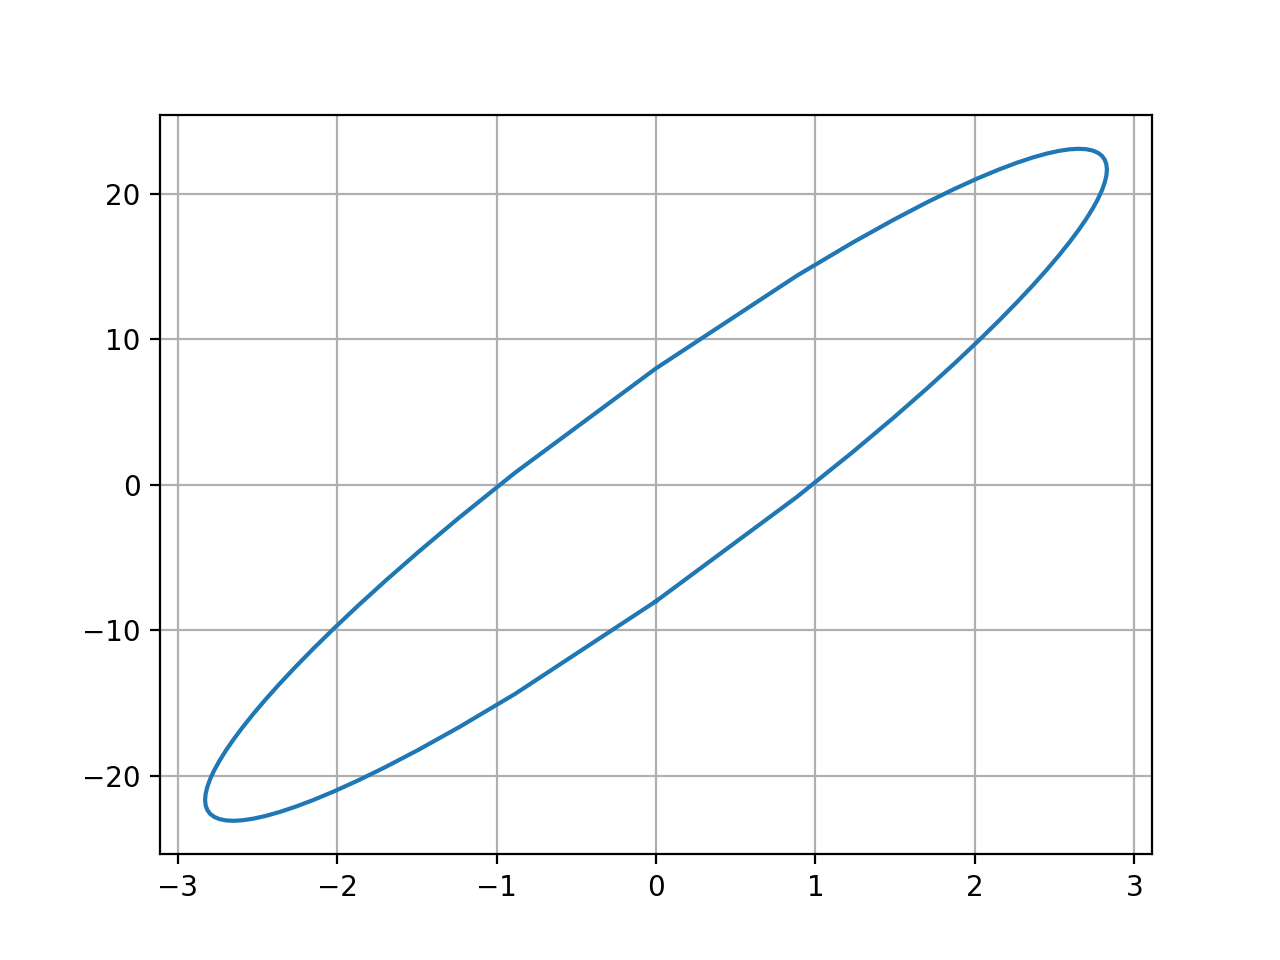
\includegraphics[width=\textwidth]{./Images/circle_scaled.png}
  \end{minipage}
\end{figure}
\end{minipage}

\pause

\begin{minipage}{0.25\textwidth}
\begin{itemize}
\item\textit{Shearing}
$$
S_k:=
\left(
\begin{matrix}
1 & k \\
0 & 1
\end{matrix}
\right)
$$
\end{itemize}
\end{minipage}  \hfill
\pause
\begin{minipage}{0.65\textwidth}
\begin{figure}[!tbp]
  \centering
  \begin{minipage}[b]{0.45\textwidth}
    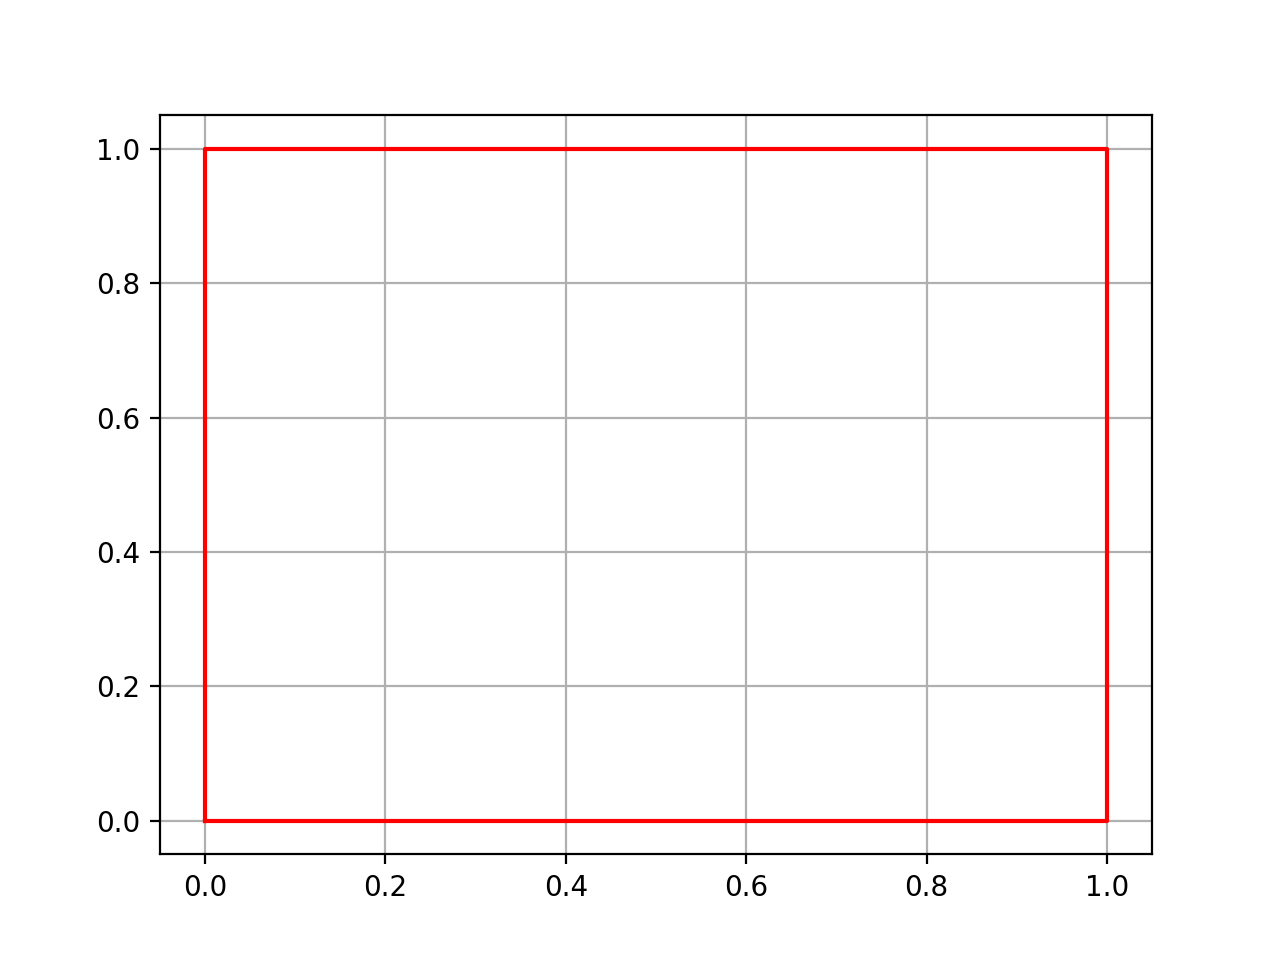
\includegraphics[width=\textwidth]{./Images/square.png}
  \end{minipage}
	\pause
 \hfill 
  \begin{minipage}[b]{0.45\textwidth}
    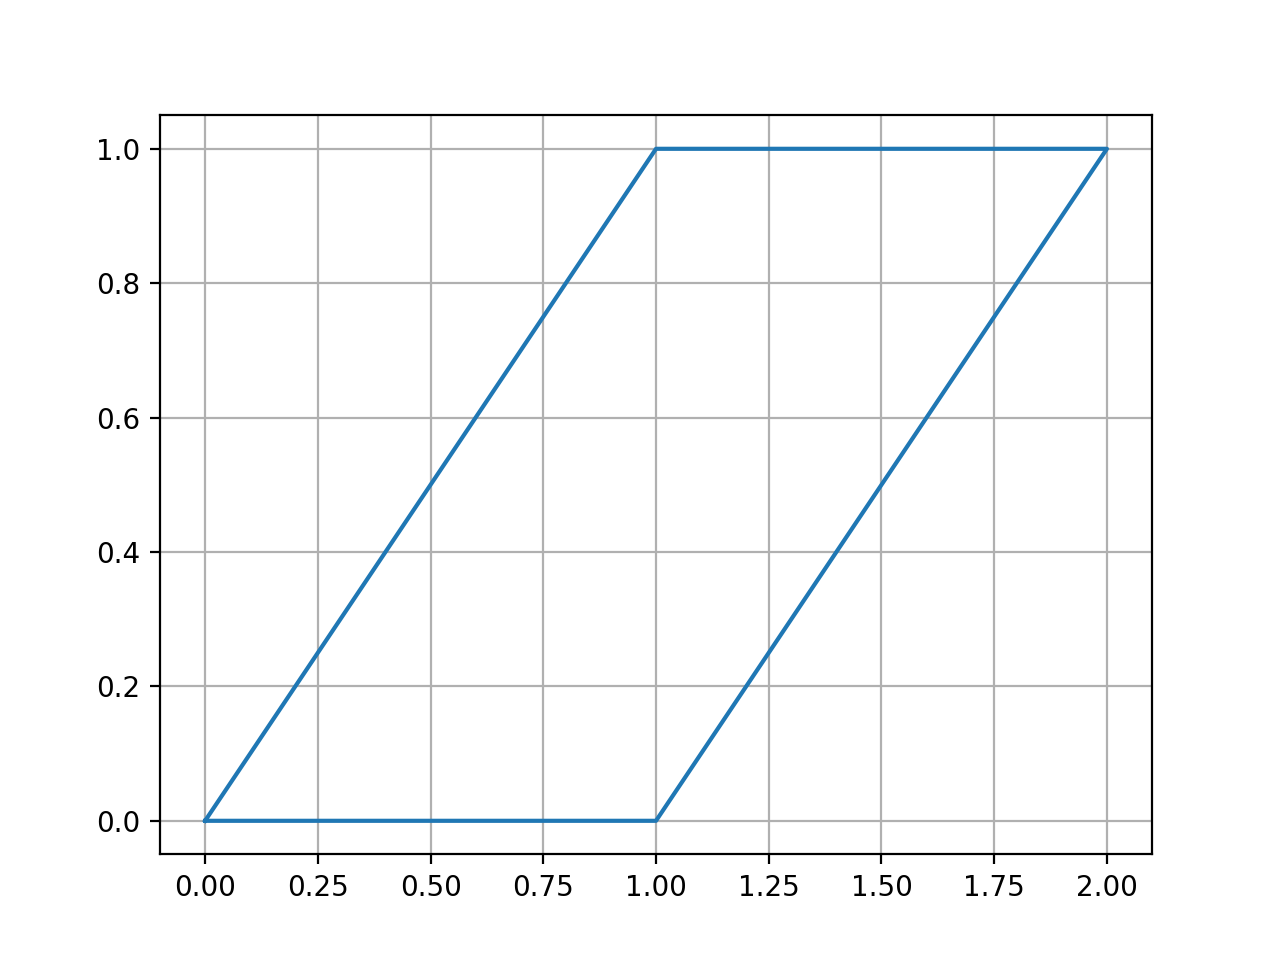
\includegraphics[width=\textwidth]{./Images/square_sheared.png}
  \end{minipage}
\end{figure}
\end{minipage}

\end{frame}

\begin{frame}{Shearlet Transform (Kutyniok, Guo, Labate, 2005)}
\begin{block}{Classical Shearlet Transform}
$$
\langle f,\psi_{j,k,m}\rangle =\int_{\mathbb{R}^2}f(x)\overline{\psi_{j,k,m}(x)}dx
$$
\pause
where
$$
\mathcal{SH}(\psi)=\{\psi_{j,k,m}(x)=2^{3j/4}\psi (S_kA_jx-m):(j,k)\in\mathbb{Z}^2,m\in\mathbb{Z}^2\}
$$
\end{block}
\pause
\begin{figure}[h!]
\centering
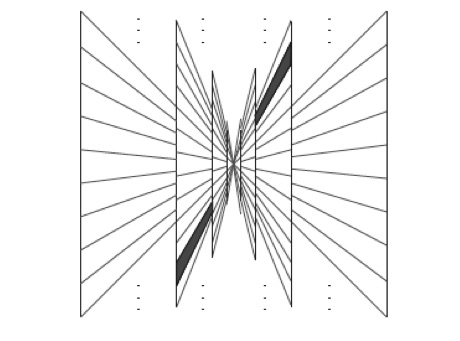
\includegraphics[width=0.4\textwidth]{./Images/tiling_nocone.jpg}
\end{figure}
\end{frame}

\begin{frame}{Cone-based shearlet transform}
$$
\mathcal{SH}(\phi,\psi,\tilde{\psi},c):=\mathcal{P}_{\mathcal{R}}\Phi(\phi,c1)\cup\mathcal{P}_{\mathcal{C}_1}\Psi(\psi,c)\cup\mathcal{P}_{\mathcal{C}_2}\tilde{\Psi}(\tilde{\psi,c})
$$
\pause
\begin{figure}[h!]
\centering
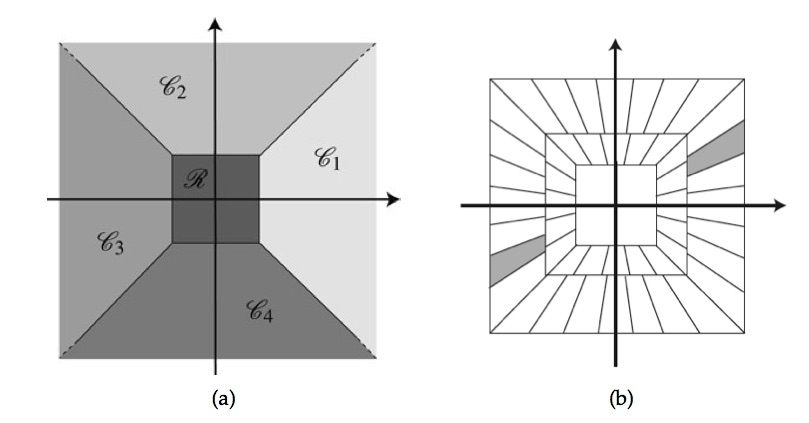
\includegraphics[width=0.9\textwidth]{./Images/tiling_cone}
\end{figure}
\end{frame}

\begin{frame}{Separable and non-separable generator}
\begin{minipage}{0.48\textwidth}
\begin{itemize}
\item\textit{Separable}
$$
\psi^{\text{sep}}(x_1,x_2)=\psi_1(x_1)\phi_1(x_2)
$$
\end{itemize}
\end{minipage}  \hfill
\pause
\begin{minipage}{0.5\textwidth}
\begin{itemize}
\item\textit{Non-separable}
$$
\hat{\psi}^{\text{non}}(\xi)=P\left(\frac{\xi_1}{2},\xi_2\right)\hat{\psi}^{\text{sep}}(\xi)
$$
\end{itemize}
\end{minipage}
\pause
\begin{figure}[h!]
\centering
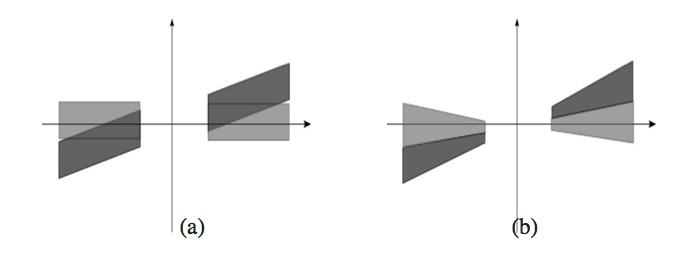
\includegraphics[width=0.7\textwidth]{./Images/separable_nonseparable}
\end{figure}
\pause
\begin{itemize}
\item Best $N$-term approximation error
$$
\sigma_N(f,\{\psi_{j,k,m}\}_{j,k,m})\sim N^{-1}(\log(N))^{3/2}
$$
\end{itemize}
\end{frame}

\begin{frame}{Current software}
\begin{itemize}
\item{Matlab}
\begin{itemize}
	\item FFST- Fast Finite Shearlet Transform (H\"auser, Steidl,TU Keiserlautern)\\ \url{http://www.mathematik.uni-kl.de/imagepro/software/ffst/}
	\item 2D/3D Shearlet Toolbox (D. Labate, University of Houston)\\ \url{https://www.math.uh.edu/~dlabate/software.html}
	\item \textbf{Shearlab3D} (G. Kutyniok, W.-Q.Lim, R. Reisenhoffer, TU Berlin)\\\url{http://www.shearlab.org/}
\end{itemize}
\pause
\item{Python}
\begin{itemize}
	\item pyShearLab (Stefan Loock, U G\"otingen) \\ \url{http://na.math.uni-goettingen.de/pyshearlab/}
\end{itemize}
\pause
\item{\textbf{Julia}}
\begin{itemize}
\item \textbf{Shearlab.jl} (H. Andrade, TU Berlin) \\ \url{https://github.com/arsenal9971/Shearlab.jl}
\end{itemize}
\end{itemize}
\end{frame}

\begin{frame}{Why Julia?}
\begin{itemize}
\item Extensive use of \lstinline[language=julia]{fft}, well implemented in Julia.

\bigskip
\pause

\item Fast vectorization and loops as well as JIT-compilation.

\bigskip
\pause
\item Plenty of image filtering, import and rescaling functions with  \lstinline[language=julia]{Images.jl, Wavelets.jl}.

\bigskip
\pause
\item Support of multithreading and painless GPU processing with  \lstinline[language=julia]{ArrayFire.jl}.
\end{itemize}
\end{frame}

\begin{frame}{Current application: Light Field Recovery}
\begin{figure}[h!]
\centering
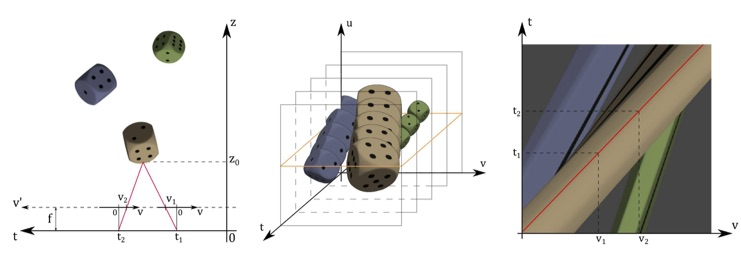
\includegraphics[width=0.9\textwidth]{./Images/dices}
\end{figure}
\pause
\begin{figure}[!tbp]
  \centering
  \begin{minipage}[b]{0.32\textwidth}
    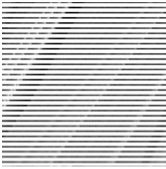
\includegraphics[width=\textwidth]{./Images/EPI_sparse}
  \end{minipage}
	\pause
 \hfill 
  \begin{minipage}[b]{0.32\textwidth}
    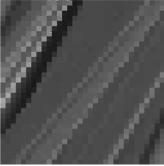
\includegraphics[width=\textwidth]{./Images/EPI_wavelet}
  \end{minipage}
\pause
	 \begin{minipage}[b]{0.32\textwidth}
    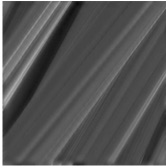
\includegraphics[width=\textwidth]{./Images/EPI_shearlet}
	\end{minipage}
\end{figure}

\end{frame}

\begin{frame}{Thanks!}
\begin{center}
\Large{Questions?}
\end{center}
\begin{figure}[h!]
\centering
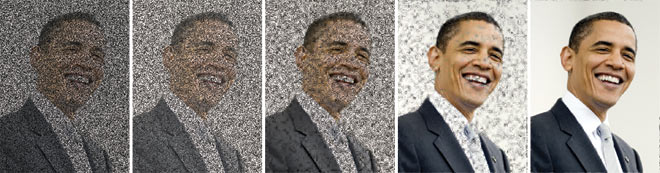
\includegraphics[width=1\textwidth]{./Images/obama_compressed.jpg}
\end{figure}
\end{frame}

